\documentclass[../analysisII_notes.tex]{subfiles}
\begin{document}
\section{Aula 07 - 26 de Março, 2025}
\subsection{Motivações}
\begin{itemize}
	\item Critérios para Existência da Integral.
\end{itemize}
\subsection{Critérios para Existência da Integral.}
Agora que demonstramos algumas propriedades das integrais superiores e inferiores, a próxima etapa é trabalhar com os critérios que garantem que uma função limitada, definida num intervalo fechado e limitado, é integrável.

O primeiro deles foi dado por Riemann e será apenas provisório, pois fundamentará o futuro critério segundo Lebesgue. Para demonstrar este critério, precisaremos de dois resultados auxiliares sobre supremo e ínfimo, junto à ideia de \textit{oscilação} de uma função num conjunto.

\begin{lemma*}
	Seja Y um conjunto limitado e não-vazio da reta real. Se M denota seu supremo e m seu ínfimo, então
	\[
		M-m = \sup_{}\{|x-y|:x, y\in Y\}.
	\]
\end{lemma*}
O que este lema quer dizer, essencialmente, é que a maior distância possível entre dois pontos dentro de Y, o chamado \textit{diâmetro} de y, é dado pela diferença entre seu supremo e seu ínfimo.
\begin{proof*}
	Primeiramente, dados elementos x e y do conjunto Y, temos
	\[
		m\leq x\leq M \quad\&\quad m\leq y\leq M \Longleftrightarrow -M\leq -y\leq -m,
	\]
	tal que
	\[
		\underbrace{m-M}_{=-(M-m)} \leq x-y \leq M-m \Rightarrow |x-y|\leq M-m,
	\]
	em que usamos a caracterização do módulo de um número pelo tamanho de um intervalo simétrico:
	\[
		|z|<r \Longleftrightarrow -r < z < r \Longleftrightarrow z\in (-r, r).
	\]

	Assim, M-m é cota superior das distâncias entre os elementos de Y; resta provar que ela é a menor das cotas superiores.

	Com efeito, dado \(\varepsilon \) positivo e elementos x, y em Y tasi que
	\[
		M-\frac{\varepsilon }{2}<M \quad\&\quad y < m + \frac{\varepsilon }{2},
	\]
	segue que
	\[
		M-\frac{\varepsilon }{2}<x \quad\&\quad -m-\frac{\varepsilon }{2}<-y \Rightarrow (M-m)-\varepsilon < x-y\leq |x-y|
	\]
	e, como os elementos são genéricos, isto significa que não existe número que seja cota superior das distâncias entre os pontos de Y e seja menor do que M-m. Portanto,
	\[
		M-m = \sup_{}\{|x-y|:\: x, y\in Y\}.\quad \text{\qedsymbol}
	\]
\end{proof*}
\begin{lemma*}
	Sejam A, B subconjuntos não-vazios da reta real tais que, para todo a em A e todo b de B, tem-se \(a\leq b\). Valem as propriedades:
	\begin{itemize}
		\item[i)] A é limitado superiormente e B é inferiormente; além disso,
		      \[
			      \sup_{}A\leq \inf_{}B;
		      \]
		\item[ii)] Há igualdade entre o supremo de A e o ínfimo de B se, e somente se, existem elementos dos conjuntos que podem ficar quão próximos um do outro quanto alguém queira:
		      \[
			      \sup_{}A = \inf_{}B \Longleftrightarrow \forall \varepsilon > 0,\: \exists \: a\in A,\:b\in B:\quad b-a<\varepsilon .
		      \]
	\end{itemize}
\end{lemma*}
\begin{proof*}
	(i) Todo elemento a em A é cota inferior de B; em contrapartida, todo elemento b de B é cota superior de A. Destas hipóteses, seguem as afirmações postuladas, bastando fixar elementos \(a_{0}\) em A e \(b_{0}\in B\), já que
	\[
		a_{0}\leq b_{0} \Rightarrow a_{0}\leq \inf_{}B.
	\]
	Como \(a_{0}\) é um elemento qualquer do conjunto A, vale que o ínfimo de B é cota superior dele, donde
	\[
		\sup_{}A\leq \inf_{}B
	\]
	por definição.

	(ii) \(\Rightarrow )\) Dado \(\varepsilon > 0\), existem elementos a, b em A e B, respectivamente, com
	\[
		a>\sup_{}A-\frac{\varepsilon }{2}\quad\&\quad b<\inf_{}B + \frac{\varepsilon }{2}.
	\]
	Rearranjando o que está escrito, temos
	\[
		\left.\begin{array}{ll}
			-a < -\sup_{}A +\frac{\varepsilon }{2} \\
			b < \inf_{}B + \frac{\varepsilon }{2}
		\end{array}\right\} \Rightarrow b-a < \overbrace{\inf_{}B-\sup_{}A}^{=0}+\varepsilon,
	\]
	mas \(\sup_{}A\) e \(\inf_{}B\) são iguais; logo, existem a em A e b em B com
	\[
		b-a < \varepsilon ,
	\]
	e a condição é cumprida.

	\(\Leftarrow )\) Reciprocamente, se a igualdade não ocorresse, o item (i) garante que deveria ser
	\[
		\sup_{}A<\inf_{}B.
	\]
	Sendo assim, como
	\[
		a\leq \sup_{}A\: \forall a\in A \quad\&\quad \inf_{}B\leq b\: \forall b\in B,
	\]
	o que resultaria é que, para todos os elementos de a e todos os de b,
	\[
		\left.\begin{array}{ll}
			\inf_{}B\leq b \\
			-\sup_{}A\leq -a
		\end{array}\right\} \Rightarrow \inf_{}B-\sup_{}A \leq b-a,
	\]
	ou seja, deveria existir um \(\varepsilon \), especificamente
	\[
		\varepsilon =\inf_{}B-\sup_{}A > 0,
	\]
	para o qual não existe elemento em a, nem em b, com
	\[
		b-a <\varepsilon.
	\]
	Portanto, esta contradição demonstra que a condição é, de fato, suficiente. \qedsymbol
	\begin{figure}[H]
		\begin{center}
			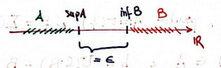
\includegraphics[height=0.5\textheight, width=0.5\textwidth, keepaspectratio]{./Images/sup_inf_07.png}
		\end{center}
		\caption{A e B estão ``separados'' por uma distância igual à diferença entre o ínfimo de B e supremo de A.}
		\label{supinf07}
	\end{figure}
\end{proof*}
\begin{def*}
	Sejam \(f:[a, b]\rightarrow \mathbb{R}\) uma função limitada e X um subconjunto com pelo menos dois pontos. Denotando por f(X) o conjunto imagem da f(x) quanto aos pontos de X, definimos a \textbf{oscilação de f no conjunto X} como o número
	\[
		\omega (f; X) = \sup_{}f(X)-\inf_{}f(X).\quad \square.
	\]
\end{def*}
Veremos futuramente que esse conceito será usado para definir uma função \(\omega:[a, b]\rightarrow \mathbb{R} \) para detectar as descontinuidades de f. Além disso, quando \(X\) é composto por um único ponto, essa definição sempre dará zero; para evitar isso, veremos o que fazer, mas depois.

Outra forma de enxergar esta definição é por meio do Lema 1, escrevendo
\[
	Y \coloneqq f(X),\: M \coloneqq \sup_{}Y,\; m\coloneqq \inf_{}Y
\]
e observando que
\[
	\omega (f; X) = \underbrace{\sup_{}Y}_{M} - \underbrace{\inf_{}Y}_{m} = \sup_{}\{|z-w|: z, w\in Y\} = \sup_{}\{|f(x)-f(y)|: x,y\in X\},
\]
dizendo que a oscilação de f em X é a maior distância entre quaisquer dois pontos da imagem de X por f. Nesse sentido, a oscilação seria um ``módulo de continuidade''.
\begin{figure}[H]
	\begin{center}
		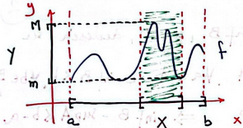
\includegraphics[height=0.5\textheight, width=0.5\textwidth, keepaspectratio]{./Images/oscilation_07.png}
	\end{center}
	\caption{note que, se X ``diminui'', \(\omega (f; X)\) também irá.}
	\label{oscilation07}
\end{figure}
\end{document}
